\subsection{The Control Plane Latency in SDN}
\label{mazu-background}

Instead of running a complex control plane on each switch, SDN delegates
network control to external applications running on a logically central
controller. 
Applications determine the routes traffic should take, and they
instruct the controller to update switches with the appropriate forwarding
state. These decisions may be based on data packets that are
received by switches and sent to the controller. Such packet events and
state update operations are enabled by OpenFlow~\cite{openflow}---a standard
API implemented by switches to facilitate communication with the controller.
Although SDN moves control plane logic from switches to a central controller, 
switches must still perform several steps to generate packet events and update
forwarding state. We describe these steps below.

\begin{figure}
\centering
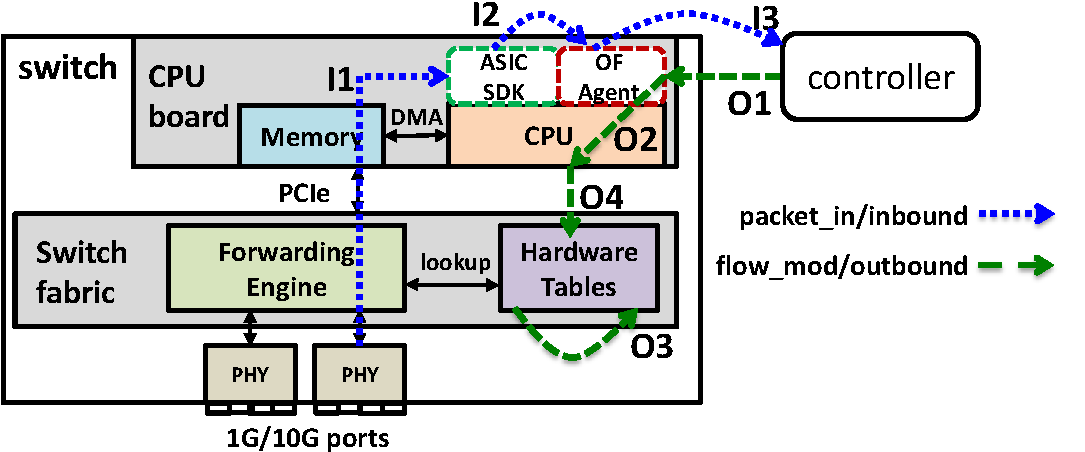
\includegraphics[width=0.55\textwidth]{figures/mazu/openflow_switch.pdf}
\caption{Schematic of an OpenFlow switch. 
We also show the factors contributing to inbound and outbound latency}\label{openflow_switch_delay}
\end{figure}

\tightparagraph{Packet Arrival} When a packet arrives, the switch ASIC first
performs a lookup in the switch's hardware forwarding tables. If a match is
found, the packet is forwarded at line rate. Otherwise the following steps
occur (Figure~\ref{openflow_switch_delay}): (I1) The ASIC sends the packet to the switch's CPU via the PCIe bus. (I2) An OS
interrupt is raised, at which point the ASIC SDK gets the packet and
dispatches it to the switch-side OpenFlow agent. (I3) The agent wakes up,
processes the packet, and sends to the controller a \packetin message
containing metadata and the first 128B of the packet. All three steps,
I1--I3, can impact the latency in generating a \packetin message. We
categorize this as {\em inbound latency}, since the controller receives the
message as input.

\tightparagraph{Forwarding Table Updates} 
The controller sends \flowmod messages to update a
switch's forwarding tables.
A switch takes the following steps to handle a \flowmod
(Figure~\ref{openflow_switch_delay}): (O1) The
OpenFlow agent running on the CPU parses the message. (O2) The agent
schedules the addition (or removal) of the forwarding rule in hardware tables, typically TCAM.  (O3)
Depending on the nature of the rule, the chip SDK may require existing rules
in the tables to be rearranged, e.g., to accommodate high priority rules.
(O4) The rule is inserted (or removed) in the hardware table.  All four steps, O1--O4,
impact the total latency in executing a \flowmod action. We categorize this
as {\em outbound latency}, since the controller outputs a \flowmod message.

\subsection{Motivating Applications}
\label{mazu-motivation-apps}

We now provide examples of management
applications that require fine-grained control over data plane state and
discuss why the control plane latency problem in SDN-enabled switches impacts
such applications. 

\tightparagraph{Failover}
It is possible that SDN can help mitigate the network-wide impact of
failures in wide-area networks, reducing both downtime and congestion
without requiring significant over provisioning. When failures occur,
the SDN management application can quickly compute new paths for flows
traversing failed nodes or links, while also simultaneously rerouting
other high/low priority flows so as to avoid hot-spots~\cite{hong2013achieving}.
However, this requires significant updates to network state at
multiple network switches. The longer these updates take, the longer
the effect of failure is felt in the form of congestion and drops. We
find that outbound latencies can inflate the time by nearly 20s
(\secref{mazu-evaluation}) putting into question SDN's applicability to
this scenario. 

\tightparagraph{Intra-Datacenter Traffic Engineering} 
Micro\-TE~\cite{benson2011microte}, Hedera~\cite{al2010hedera}, 
and other recent proposals have
argued for using SDN to route traffic subsets at fine time-scales in order to
achieve fine-grained traffic engineering in data centers. For instance,
MicroTE leverages the fact that a significant fraction of ToR-to-ToR DC
traffic (ToR is ``top-of-rack'' switch) is predictable on short time-scales
of 1-2s. It computes and installs at ToR switches routes for such traffic
on short time-scales. % The computed routes may only be effective for 1-2s
% after which a new sets of routes may be more optimal. 
Thus, latencies in installing routes can significantly undermine MicroTE's
effectiveness. Indeed, we find that updating a set of routes at a ToR switch
in MicroTE can take as long as 0.5s on some SDN switches
(\secref{mazu-evaluation}). 
